\subsection{Sphere-line picking}
\label{sec:sphere_line}

Sphere-line picking is subtly different from ball-line picking. In
this new case, we choose points on the surface of a 2-sphere (the
sphere in 3D), but the lines are straight lines in the 3D space in
which the sphere is embedded, i.e., we use the standard Euclidean
distance metric.

The $2$-sphere is the set of points $S^n = \big\{ {\mathbf x} \in \R^2
\; \big| \; \|{\mathbf x} \|_2 \leq R \big\},$ where $R$ is the {\em
  radius}.
% http://en.wikipedia.org/wiki/N-sphere

Figure~\ref{fig:sphere_eg} shows an example of the line-picking
problem on the 2-sphere. Generating points uniformly on the sphere
requires a little care: it can be accomplished by taking 
\begin{equation}
    \label{eq:x_surface_sphere2}
    \x = R \frac{\y}{\| \y \|_2}, 
\end{equation}
where the $y_i \sim N(0,1)$ are IID standard normal random variates.
The result is a set of points chosen so that the probability of there
being $k$ points inside non-overlapping regions of are $a$ takes
IID Poisson distributions with mean $\lambda a$ where $\lambda =
m/V_n$, where $m$ is the total number of points generated, and $S_2$
is the surface area of the sphere.

\begin{figure}[tbp]
  \begin{center}
    \subfloat[\label{fig:sphere_eg}2-ball
    example.]{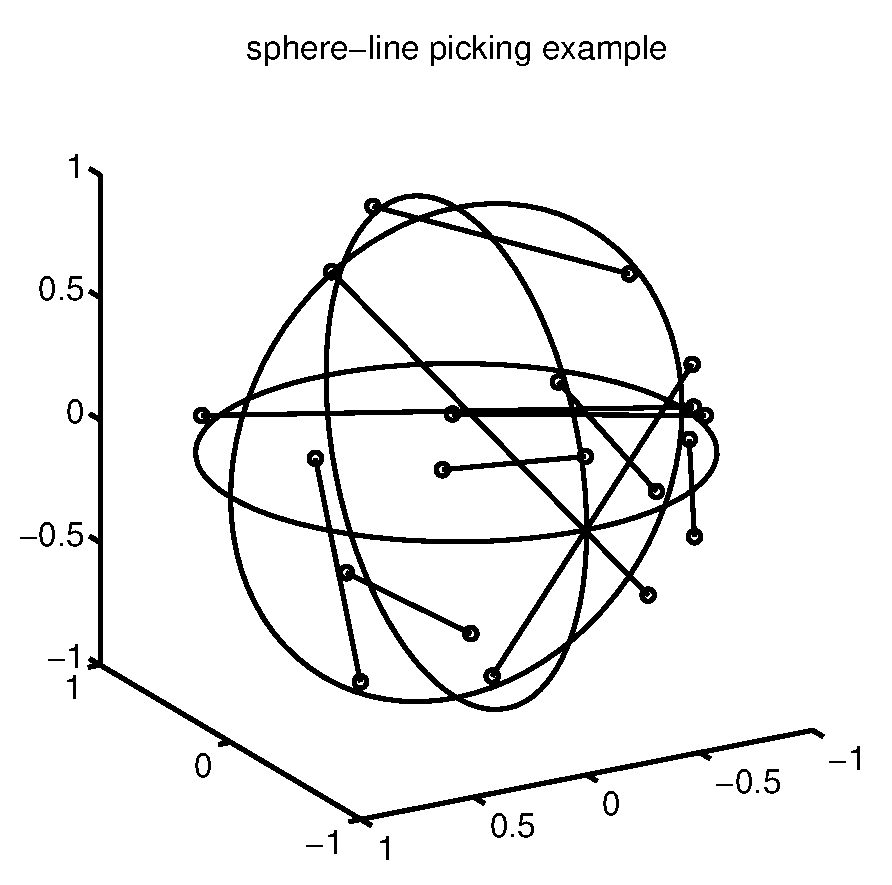
\includegraphics[width=0.4\columnwidth]{../Matlab/Plots/LinePicking_test_sim_sphere_eg.eps}} 
    \hspace{6mm}
    \subfloat[\label{fig:sphere_pdf}PDF of $n$-balls.]{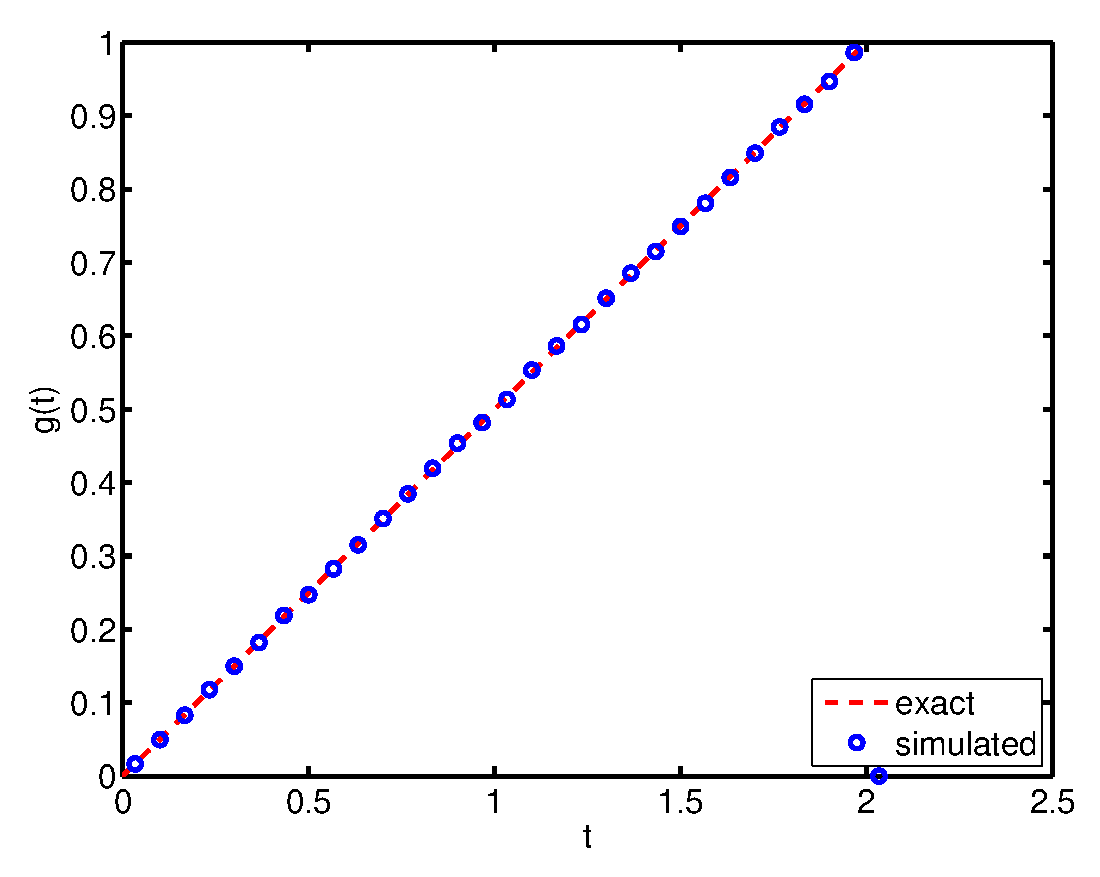
\includegraphics[width=0.48\columnwidth]{../Matlab/Plots/LinePicking_test_sim_sphere.eps}}
    \caption{The sphere-line picking problem.}
  \end{center} 
\vspace{-4mm}
\end{figure}

\subsubsection{PDF}



The PDF is unusual in that it, and the line-line picking problem CDFs
are exactly opposite (and these are the only two that have their mode
at one end of the support, i.e., these are the only two monotonic
densities.

\subsubsection{CDF}


\subsubsection{Moments}
